\documentclass[12pt,a4paper]{article}

\usepackage{graphicx}
\usepackage{abstract}
\usepackage{wrapfig}
\usepackage{mathrsfs,amsmath} 
\usepackage{geometry}
\usepackage{fancyhdr}
\usepackage[T1]{fontenc}
\usepackage[polish]{babel}
\usepackage[utf8]{inputenc}
\usepackage{lmodern}
\usepackage{listings}
\usepackage{color}
\usepackage{xcolor}
\usepackage{hyperref}
\usepackage{subcaption}
\usepackage{multicol}
\usepackage{cleveref}
\usepackage{siunitx}

\setlength{\headheight}{12pt} 
\setlength{\textheight}{25cm}
\setlength{\textwidth}{17cm}
\setlength{\footskip}{10mm}
\setlength{\oddsidemargin}{0mm}
\setlength{\evensidemargin}{0mm}
\setlength{\topmargin}{0mm}
\setlength{\headsep}{10mm}

\lstdefinestyle{mystyle}{
    backgroundcolor=\color{backcolour},   
    commentstyle=\color{codegreen},
    keywordstyle=\color{magenta},
    numberstyle=\tiny\color{codegray},
    stringstyle=\color{codepurple},
    basicstyle=\footnotesize,
    breakatwhitespace=false,         
    breaklines=true,                 
    captionpos=b,                    
    keepspaces=true,                 
    numbers=left,                    
    numbersep=5pt,                  
    showspaces=false,                
    showstringspaces=false,
    showtabs=false,                  
    tabsize=2
}
 
\definecolor{codegreen}{rgb}{0,0.6,0}
\definecolor{codegray}{rgb}{0.5,0.5,0.5}
\definecolor{codepurple}{rgb}{0.58,0,0.82}
\definecolor{backcolour}{rgb}{0.95,0.95,0.92}
\lstset{style=mystyle}

\selectlanguage{polish}

\newgeometry{rmargin=2.5cm,lmargin=2.5cm,bmargin=2.5cm}
\pagestyle{fancy}
\rhead{Fizyka Techniczna}
\chead{}
\lhead{}
\lfoot{}
\cfoot{\thepage  }
\rfoot{}

\begin{document}

\thispagestyle{empty}
\begin{center}
{\Large \textbf{Fizyka Fazy Skondensowanej}}
\end{center}
\newpage

\tableofcontents
\newpage

\section{Zestaw:}
\subsection{Pierwszy}
\subsubsection{}
\begin{enumerate}
\item Sieć  krystaliczna, węzły sieci, proste sieciowe, płaszczyzny sieciowe, wskaźniki Millera (hkl), Komórka elementarna i  typy układów krystalograficznych
\item Operacje symetrii, grupy punktowe.
\item Sieć prosta a sieć odwrotna. Objętości komórki elementarnej w sieci odwrotnej. Odległości międzypłaszczyznowe. Strefy Brillouina.
\end{enumerate}
\subsubsection*{Rozwiązanie:}


\subsubsection{}
Obliczyć objętość komórki elementarnej dla układu regularnego, romboedrycznego, heksagonalnego, jednoskośnego.
\subsubsection*{Rozwiązanie:}

\subsubsection{}
Wykaż, że:
\begin{enumerate}
\item dla prostej sieci regularnej o stałej sieciowej $a$, odległość międzypłaszczyznowa \[d^2_{hkl} =\frac{a^2}{h^2+k^2+l^2}\] 
\item obliczyć $\frac{1}{d^2_{hkl}}$ dla układu heksagonalnego oraz rombowego
\end{enumerate}
\subsubsection*{Rozwiązanie:}

\subsubsection{}
Struktura diamentu zawiera dwa identyczne atomy w położeniach $000$ i $\frac{1}{4}\frac{1}{4}\frac{1}{4}$ związane z każdym węzłem sieci powierzchniowo centrowanej \textit{(fcc)}. Obliczyć czynnik strukturalny dla tej struktury. Pokaż, że dozwolone odbicia spełniają warunek $h + k + l = 4n$, gdzie wszystkie wskaźniki są parzyste, a $n$ jest dowolna liczbą całkowitą, albo wszystkie składniki są nieparzyste.  
\subsubsection*{Rozwiązanie:}

\newpage

\subsection{Drugi}
\subsubsection{}
Energia oddziaływania między dwoma atomami w cząsteczce opisywana jest wzorem:
\[U(r) = -\frac{\alpha}{r^n}+\frac{\beta}{r^m}\]
Pokazać, że $m>n$.
\subsubsection*{Rozwiązanie:}
pierwsza pochodna:
\begin{equation}
\frac{\partial U}{\partial r} = \frac{n\alpha}{r^{n+1}} - \frac{m\beta}{r^{m+1}}=0 \rightarrow \frac{n\alpha}{r^{n+1}} = \frac{m\beta}{r^{m+1}}
\end{equation}
\begin{equation}
\label{eq:pp}
\frac{r^{m+1}}{r^{n+1}} = r^{m-n} = \frac{m\beta}{n\alpha}
\end{equation}
druga pochodna:
\begin{equation}
\frac{\partial^2 U}{\partial r^2} = - \frac{n(n+1)\alpha}{r^{n+2}} + \frac{m(m+1)\beta}{r^{m+2}} > 0
\end{equation}
\[ \frac{n(n+1)\alpha}{r^{n+2}} < \frac{m(m+1)\beta}{r^{m+2}} \]
\[n(n+1)\alpha \left( \frac{r^{m+2}}{r^{n+2}} \right) = n(n+1)\alpha r^{m-n} < m(m+1)\beta\]
z (\ref{eq:pp}):
\[ n(n+1)\alpha \frac{m\beta}{n\alpha} = (n+1)m\beta = nm\beta + m\beta < m^2\beta + m\beta\]
\[nm < m^2 \rightarrow n<m\]
\hrulefill

\subsubsection{}
Rozważ liniowy układ $2N$ jonów o ładunku równym na przemian $\pm q$. Załóż, że energia potencjalna odpychania między najbliższymi sąsiadami ma postać $\frac{A}{R^n}$. 
\begin{enumerate}
\item Pokaż, że dla odległości między jonami odpowiadającej stanowi równowagi 
\[U(R_0) = -\frac{2Nq^2\ln(2)}{R_0}\left(1-\frac{1}{n}\right)\]
\item Załóżmy, że kryształ został ściśnięty tak, że $R_0\rightarrow R_0(1-\delta)$. Pokaż, że w wyrażeniu na pracę związaną ze ściśnięciem kryształu największy wkład opisuje człon $\frac{C\delta^2}{2}$ gdzie:
\[C=\frac{(n-1)q^2\ln(2)}{R_0}\]
\end{enumerate}
\subsubsection*{Rozwiązanie:}
\begin{enumerate}
\item Energia potencjalna oddziaływania między dwoma atomami dana jest przez:
\begin{equation}
\label{eq:UR}
U(R) = N\left( \frac{A}{R^n} - \frac{\alpha q^2}{R} \right)
\end{equation}
gdzie $\alpha$ jest stałą Madelunga wynoszącą dla przypadku liniowego $\alpha = 2\ln 2$.\\
Dla stanu równowagi spełniony musi być warunek:
\begin{equation}
\frac{\partial U}{\partial R} = 0
\end{equation}
stąd:
\begin{equation}
\frac{\partial U}{\partial R} = N \left( -\frac{nA}{R_0^{n+1}} + \frac{\alpha q^2}{R_0^2} \right)= 0
\end{equation}
\begin{equation}
\label{eq:dudr}
\frac{nA}{R_0^{n+1}} = \frac{\alpha q^2}{R_0^2} \rightarrow \frac{A}{R_0^n} = \frac{\alpha q^2}{n R_0}
\end{equation}
Wstawiając wyrażenie (\ref{eq:dudr}) do (\ref{eq:UR}) oraz $\alpha=2\ln(2)$ otrzymuje się:
\begin{equation}
U(R_0) = N \left( \frac{\alpha q^2}{R_0^n} - \frac{\alpha q^2}{R_0} \right) = \frac{2Nq^2\ln(2)}{R_0} \left( \frac{1}{n} -1 \right)
\end{equation}
\hrulefill
\item yyy
\end{enumerate}

\subsubsection{}
Obliczyć stałą Madelunga dla kryształu \textit{NaCl}:
\begin{enumerate}
\item przypadek jednowymiarowy (nić krystaliczna \textit{NaCl})
\begin{figure}[h!]
\centering
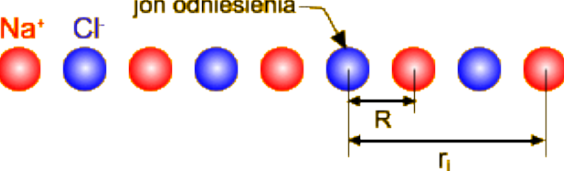
\includegraphics[scale=0.3]{images/zes2-1}
\end{figure}
\item przypadek dwuwymiarowy (siatka płaska \textit{NaCl})
\begin{figure}[h!]
\centering
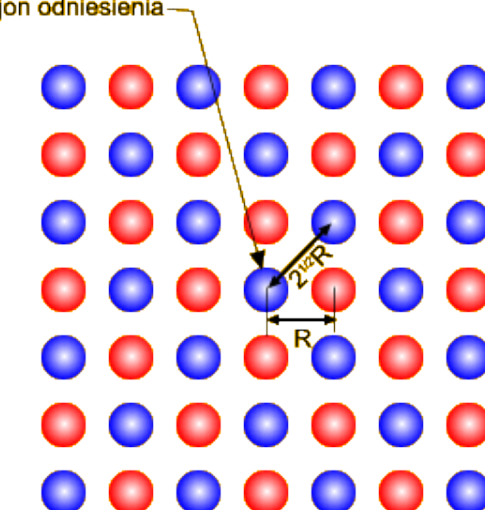
\includegraphics[scale=0.5]{images/zes2-2}
\end{figure}
\end{enumerate}
\subsubsection*{Rozwiązanie:}
\textbf{przypadek 1}
Stała Madelunga jest używana do wyznaczania potencjału elektrostatycznego pojedynczych jonów w krysztale, przez zbliżanie się jonów przez ładunki punktowe. 
\\
\\
wzór ogólny:
\\
\\
\begin{equation}
\alpha=\sum \frac {\pm}{p_i}
\end{equation}
\\
\\
W naszym przypadku: 
\\
\\
\begin{equation}
\frac{\alpha}{R}=2\left( \frac{1}{R}-\frac{1}{2R}+\frac{1}{3R}-\frac{1}{4R}+\frac{1}{5R} \right)
\end{equation}
\\
gdzie jako jon odniesienia bierzemy jon zaznaczony na rysunku, następnie odejmujemu lub dodajemy w zależności od znaku jonu w minaowniku są wielokrotności odległości od jonu odniesienia.
\\
\\
Używając rozwinięcia w szereg Maclurina możemy udowodnić, że szereg:
\\
\\
\begin{equation}
x-\frac{x^2}{2}+\frac{x^3}{3}-\frac{x^4}{4}....
\end{equation}
\\
\\
którego wzór ogólny ma postać:
\\
\\
\begin{equation}
\sum_{n=1}^{\infty}\frac{(-1)^{n+1}}{n}x^n
\end{equation}
\\
\\
jest zbierzny do funkcji ln(1+x), gdzie x=1.
\\
\\
Rozwinięcie:
\\
\\
$f(x)=ln(x+1)$   =>   $f(0)=ln(1)=0$
\\
\\
$f'(x)=-\frac{1}{(x+1)^2}$   =>   $f(0)=-1$
\\
\\
$f''(x)=\frac{2}{(x+1)^3}$   =>   $f(0)=2$
\\
\\
$f'''(x)=-\frac{6}{(x+1)^5}$   =>   $f(0)=-6$
\\
\\
$=0+1*\frac{x}{1}-1*\frac{x^2}{2}+\frac{x^3}{6}-\frac{x^4}{4}$
\\
\\
ogólny wynik:
$\alpha=2ln2$
\\
\\
\textbf{przypadek drugi}
\\
\\
Odległości obliczmy w natępujący sposób:
\\
\\
-jako jon odniesienia bierzemy jon w środku.
\\
\\
-dzielimy przestrzeń na cztery kwadraty i wszystko liczmy dla jednego kwadratu potem mnożymy razy cztery.
\\
\\
-pierwsze trzy wartości w nawiasie są to odległości od jonu odniesienia w prawo (liczmy je tak jak poprzednio, w liczniku znak, a wmianowniku wielokrotność odległości od jonu odniesienia)
\\
\\
-następnie liczmy odległość jonu oznaczone gwiazdką, mnożymy przez odpowiedni znak i dodajemy do sumy (liczmy ze wzoru Pitagorasa)
\\
\\
następnie liczmy odległości dwóch jonów oznaczonych paprykami i mnożymy razy dwa ponieważ na prawo od jonu z gwiazdką też mamy papryki.
\\
\\
-potem liczymy jony oznaczone słońcami 
\\
\\
-a na końcu jon oznaczony prostokątem i mnożymy razy dwa bo po prawej też jest prostokąt.
\\
\\
I wychodzi nam:
\\
\\
\begin{equation}
\frac{\alpha}{R} =\frac{4}{R}(1-\frac{1}{2}+\frac{1}{3}-\frac{1}{\sqrt{2}}=\frac{2}{\sqrt{5}}-\frac{2}{\sqrt{10}}-\frac{1}{2\sqrt{2}}-\frac{1}{3\sqrt{2}}+\frac{2}{\sqrt{13}})
\end{equation}
\\
\\
opisane wyżej odległości, które znajdują się w licznikach liczymy ze wzoru pitagorasa, np. dla jonu z gwiazdką:
\\
\\
\begin{equation}
R^2+R^2=R^2
\end{equation}
\begin{equation}
2R^2=R^2
\end{equation}
\begin{equation}
R=\sqrt{2}R
\end{equation}

\subsubsection{}
Obliczyć jakie ciśnienie należy przyłożyć do kryształu jonowego, aby odległość między jonami zmniejszyła się o $1$ procent.
\subsubsection*{Rozwiązanie:}

\subsection{Trzeci}
\subsubsection{}
Poniższy rysunek przedstawia temperaturową zależność oporu elektrycznego. Określ, czy jest to zależność dla metali czy izolatorów. Opisz proces fizyczny, który opisuje tą zależność w zakresie temperatur: 
a) blisko 0 K, 
b) około 25 K, 
c) około 300 K. 
Oszacuj średnią drogę swobodną i czas w $T = 0$K i $T = 300$K. Przydatne stałe: $n = 10^{23} cm^{-3}$, $m = 10^{27}$kg, $v_f = 108 \frac{cm}{s}$, $e = 4.8 \cdot 10^{10} $esu $(e = 1,6^{19} C)$, $1(\Omega cm)^2 = 9 \cdot 10^{11}$esu.
\subsubsection*{Rozwiązanie:}


\subsubsection{}
\begin{figure}[h]
\centering
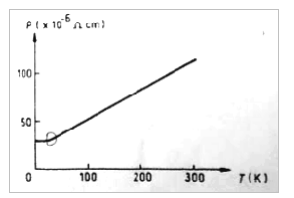
\includegraphics[scale=0.7]{images/zes3-2}
\end{figure}
\subsubsection*{Rozwiązanie:}


\subsubsection{}
Rozpatrzyć falę podłużną $u_s=u(0)\cos{(\omega t -sKa)}$, która rozchodzi się w jednoatomowej sieci liniowej składającej się  z atomów o masach $M$ odległych od siebie o $a$; stała siłowa oddziaływania między najbliższymi sąsiadami wynosi $C$.
\begin{itemize}
\item Wykazać, że całkowita energia fali wynosi:
\[E = \frac{1}{2}M \sum_s \left(\frac{du_s}{dt}\right)^2 + \frac{1}{2}C\sum_s(u_s - u_{s+1})^2\]
\item Podstawiając wyrażenie na $u_s$ do powyższego wzoru wykaż, że uśredniona w czasie energia całkowita przypadająca na jeden atom wynosi:
\[\frac{1}{4}M\omega^2 u^2(0) + \frac{1}{2}C(1-cos(Ka))u^2(0) = \frac{1}{2} M \omega^2 u^2(0)\]
\end{itemize}
\subsubsection*{Rozwiązanie:}
\textbf{podpunkt a}

fala podłużna: 

\begin{equation}
U_s=U cos(\omega-ska)
\end{equation}

a-odległość pomiędzy atomami,
$\omega$-częstotliwość,
s-pozycja atomu,
$k=\frac{2\pi}{\lambda}$
\\
\\
prędkość:
\\
\begin{equation}
v=\frac{dU_s}{dt}=\frac{d}{dt}(Ucos(\omega t- ska)
\end{equation}
\\
\\
energia kinetyczna:
\\
\begin{equation}
E_k=\frac{1}{2}Mv^2=\frac{1}{2}M(\frac{dU_s}{dt})^2
\end{equation}
\\
\\
całkowita energia kinetyczna fali- suma energi poszczególnych atomów:
\\
\\
\begin {equation}
E_k=\sum\frac{1}{2}M(\frac{dU_s}{dt})^2
\end{equation}
\\
\\
energia potencjalna:
\\
\\
\begin{equation}
E_p=\frac{1}{2}kx^2-> \frac{1}{2}C(U_s-U_{s+1})^2
\end{equation}
\\
c-stała siłowa
\\
\\
całkowita energia potencjalna:
\\
\begin{equation}
E_p=\sum\frac{1}{2}kx^2-> \frac{1}{2}C(U_s-U_{s+1})^2
\end{equation}
\\
\\
całkowita energia:
\\
\begin{equation}
E=\frac{1}{2}\sum M(\frac{dU_s}{dt})^2+\frac{1}{2}C\sum(U_s-U_{s+1})^2
\end{equation}
\\
\\
\\
\textbf{podpunkt b}
\\
\\
$U_s=Ucos(\omega t-ska)$
\\
$U_{s+1}=Ucos(\omega t-(s+1)ka)$
\\
\\
korzystamy z zależności $cos(\alpha - \beta)=cos\alpha cos\beta+sin\alpha sin\beta$
\\
\\
$U_{s+1}=U[cos(\omega t- ska-ka]=U[cos(\omega t-ska)cos(ka)+sin(\omega t-ska)sin(ka)]$
\\
\\
$U_s-U_{s+1}=Ucos(\omega t-ska)-U[cos(\omega t- ska-ka]=U[cos(\omega t-ska)cos(ka)+sin(\omega t-ska)sin(ka)]$
\\
\\
$=Ucos(\omega t-ska)[1-cos(ka)]+sin(\omega t-ska)sin(ka)]$
\\
\\
$E=\frac{1}{2}M(\frac{d}{dt}Ucos(\omega t-ska)^2+\frac{1}{2}C[Ucos(\omega t-ska)[1-cos(ka)]+sin(\omega t-ska)sin(ka)]^2$
\\
\\
$=\frac{1}{2}M[-U\omega sin(\omega t-ska]^2+\frac{1}{2}C[Ucos(\omega t-ska)[1-cos(ka)]+sin(\omega t-ska)sin(ka)]^2$
\\
\\
podstawiamy:
\\
\\
$\omega t-ska -> A$
\\
$ka ->B$
\\
\\
$E=\frac{1}{2}M[-u\omega sinA]^2+\frac{1}{2}CU^2[cosA(1-cosB)+sinAsinB]^2$
\\
\\
$=\frac{1}{2}M\omega^2U^2sin^2A+\frac{1}{2}CU^2[cos^2A(1-cosB)^2+sin^2Asin^2B+2cosA(1-cosB)sinAsinB$
\\
\\
$=\frac{1}{2}M\omega^2U^2sin^2A+\frac{1}{2}CU^2[cos^2A(1-2cosB+cos^2B)+sin^2AB+2cosA(1-cosB)sinAsinB$
\\
\\
$=\frac{1}{2}M\omega^2U^2sin^2A+\frac{1}{2}CU^2[cos^2A-2cos^2AcosB+cos^2Acos^B+sin^2Asin^2B+2cosA(1-cosB)sinAsinB$
\\
\\
$<cos^2>=\frac{1}{2}$
\\
$<sin^2>=\frac{1}{2}$
\\
$<sin cos>=0$
\\
\\
$E=\frac{1}{2}M\omega^2U^2\frac{1}{2}+\frac{1}{2}CU^2[\frac{1}{2}-cosB+\frac{1}{4}+\frac{1}{4}+2*0*sinB-2*0*0]$
\\
\\
$=\frac{1}{4}M\omega^2U^2+\frac{1}{2}CU^2[\frac{1}{2}-cosB+\frac{1}{2}]=\frac{1}{4}M\omega^2U^2+\frac{1}{2}[1-cosB]$
\\
\\
B->ka
\\
\\
$E=\frac{1}{4}M\omega^2U^2+\frac{1}{2}CU^2(1-cos(ka)$
\\
\\
relacja dyspersyjna:
\\
\\
$\omega^2=\frac{2C}{M}(1-cos(ka))$
\\
\\
$\frac{M\omega^2}{2C}=(1-cos(ka))$
\\
\\
$E=\frac{1}{4}M\omega^2U^2+\frac{1}{4}U^2\frac{M\omega^2}{2}$
\\
\\
$E=\frac{1}{2}M\omega^2U^2$

\subsubsection{}
Wyznaczyć podłużny fonon akustyczny oraz widmo optyczne dla sieci liniowej o stałej a zawierającej w komórce dwa jednakowe atomy o masach $M$, których odległość w położeniu równowagi wynosi $\delta < \frac{1}{a}$.
\subsubsection*{Rozwiązanie:}
\subsubsection*{Rozwiązanie:}


\subsubsection{}
Dana jest sieć:
\begin{figure}[h!]
\centering
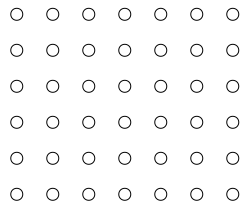
\includegraphics[scale=0.9]{images/zes3-5}
\end{figure}
\begin{itemize}
\item Wykazać. że
\[M\frac{d^2u_{lm}}{dt^2} = C\big( (u_{l+1,m} - u{l-1,m} - 2u_{lm}) + (u_{l,m+1} - u_{l,m-1} -2u_{lm}) \big)\]
\item Przyjąć: $u_{lm} = u(0) \exp\big( i(lK_xa + mK_ya - \omega t) \big)$ i wykazać, że:
\[ \omega^2 M= 2C(2-\cos (K_xa) - \cos(K_ya) ) \]
\item Wykazać, że przedział wartości wektora $K$, dla których istnieją niezależne rozwiązania można przyjąć kwadrat o baku $\frac{2\pi}{a}$
\item Dla $Ka <<1$ wykazać, że:
\[ \omega = \left( \frac{Ca^2}{M} \right)^{\frac{1}{2}} \big( K_x^2 + K_y^2 \big) = \left( \frac{Ca^2}{M} \right) K \]
\end{itemize}
\subsubsection*{Rozwiązanie:}


\subsection{Czwarty}
\subsubsection{}
\label{subsubsec:41}
Wyprowadzić wzory na funkcję gęstości stanów dla łańcucha jednoatomowego zakładając, że $\omega = \upsilon \cdot k$. Określić częstotliwość Debye'a.
\subsubsection*{Rozwiązanie:}
\textbf{funkcja gęstości stanów}
D$(\omega)$ jest to liczba modów różnych dragań przypadająca na jednostkowy zakres częstotliwości.
\\
\\
przemieszczenia atomu w drganiach podłuznych i poprzecznych określa zależność:
\\
\\
$U_s ~sin(sKa)$
\\
\\
dobieramy tak wartości K żeby atomy na końcu i początku łańcucha były unieruchomione.
\\
wartości wektora falowego, które są dozwolone:
\\
\\
K= +/-$\frac{2\pi}{L},\frac{4\pi}{L},.....$
\\
Gęstość stanów opisuje wzór:
\\
\\
\begin{equation}
D(\omega)=\frac{dN}{d\omega}
\end{equation}
\\
gdzie N to całkowita liczba modów drgań o wartości wektora falowego mniejszego od k.
\\
\\
$K=\frac{N\pi}{L}$
\\
\\
$N=\frac{KL}{N}$
\\
\\
$D(\omega)=\frac{d}{d\omega}\frac{KL}{\pi}=\frac{L}{\pi}\frac{dK}{d\omega}=\frac{L}{\pi v}=\frac{L K}{\pi \omega}$
\\
\\
gdzie $\frac{dK}{d\omega}$ - prędkość grupowa, $k=\frac{\omega}{v}$
\\
\\
częstotliwość Debaya jest to teoretyczna najwyższa możliwa częstotliwość drgań atmów  wsieci krystalicznej.
\\
\\
$N=\frac{KL}{\pi}=\frac{\omega L}{v\pi}$
\\
\\
$\omega_D=\frac{Nv\pi}{L}$




\subsubsection{}
\label{subsubsec:42}
Wyprowadzić wzory na funkcję gęstości stanów dla sieci kwadratowej zakładając, że $\omega = \upsilon \cdot k$. Określić częstotliwość Debye'a.
\subsubsection*{Rozwiązanie:}


\subsubsection{}
Korzystając z wyników zadań \ref{subsubsec:41} i \ref{subsubsec:42} wyprowadzić wzory na molowe ciepło właściwe.
\subsubsection*{Rozwiązanie:}


\subsubsection{}
\label{subsubsec:44}
Znaleźć zależność poziomu Fermiego w temperaturze zera bezwzględnego od gęstości elektronowej $n$:
\[E_F(T=0) = \frac{\hbar^2}{2m}(3n\pi^2)^{\frac{2}{3}}\]
oraz zależność średniej energii na elektron od energii Fermiego.
\[ \overline{E}(T=0) = \frac{3}{5}E_F \]
\subsubsection*{Rozwiązanie:}
Energia Fermiego dana jest wzorem:
\begin{equation}
\label{eq:E_F}
E_F = \frac{\hbar^2}{2m}k_F^2
\end{equation}
Na każdy element objętości $v_1 = \left(\frac{2\pi}{L}\right)^2$ przypada jeden wektor falowy $k$.\\
Stąd dla objętości $v_2 = \frac{4}{3}\pi k_F^3$ całkowita liczba stanów wynosi($2$ dozwolone stany spinowej liczby kwantowej):
\begin{equation}
N = 2 \frac{v_2}{v_1} = 2 \frac{4\pi k_F^3 L^3}{3\cdot 8 \pi^3} =  \frac{V}{3\pi^2}k_F^3
\end{equation}
czyli
\begin{equation}
\label{eq:k_F}
k_F = \left( \frac{3 \pi^2 N}{V} \right)^{\frac{1}{3}} =  (3\pi n)^{\frac{1}{3}}
\end{equation} 
gdzie gęstość stanów $n = \frac{N}{V}$.\\
Podstawiając wyrażenie (\ref{eq:k_F}) do równania (\ref{eq:E_F}) otrzymuje się:
\begin{equation}
E_F = \frac{\hbar^2}{2m} (2n\pi)^{\frac{2}{3}}
\end{equation} 
\hrulefill
\newline
W przypadku 1D energia elektronu w stanie $n$ wynosi:
\begin{equation}
E_n = \frac{\hbar^2 \pi^2}{2mL^2}n^2
\end{equation}
Dla  $N$ poziomów śrenią energię można wyrazić przez:
\begin{equation}
\overline{E} = 2 \frac{\sum^N E_n}{2N}
\end{equation}
gdzie energia ostatniego elektronu jest enegią Fermiego:
\begin{equation}
\label{eq:E_F2}
E_F = \frac{\hbar^2 \pi^2}{2mL^2} N^2
\end{equation}
Stosując przybliżenie:
\begin{equation}
\sum^N_{n=1} n^2 = \frac{1}{6}(2N^2 + 3N + 1) = \frac{N^3}{3} + \frac{N^2}{2} + \frac{N}{6} \sim \frac{N^3}{3}
\end{equation} 
oraz (\ref{eq:E_F2}), średnia energia elektronu wyraża się przez:
\begin{equation}
\overline{E} = \frac{2}{2N} \frac{\hbar^2 \pi^2}{2mL^2} \sum^N n^2 = \frac{2}{2N} \frac{\hbar^2 \pi^2}{2mL^2} \frac{N^3}{3} = \frac{1}{3} E_F
\end{equation}





\subsubsection{}
Wyprowadzić wzór na funkcję gęstości stanów elektronów swobodnych w przypadku jednowymiarowym.
\subsubsection*{Rozwiązanie:}


\subsubsection{}
Wyprowadzić wzór na funkcję gęstości stanów $g(E)$  gazu elektronowego dla sieci kwadratowej.
\subsubsection*{Rozwiązanie:}
Pole koła: $\pi k_f^2$
\\
\\
element powierzchni: $(\frac{2\pi}{L})^2$
\\
\\
\begin{equation}
N=\frac{L^2k_f^2}{4\pi}
\end{equation}
\\
\begin{equation}
f_f=\frac{4\pi N}{L^2} 
\end{equation}
\\
\begin{equation}
E_f=\frac{\hbar^2}{2m}\frac{4\pi N}{L^2}
\end{equation}
\\
\begin{equation}
N=\frac{mL^2E_f}{2\pi \hbar^2}
\end{equation}
\\
\begin{equation}
\frac{dN}{d\omega}=frac{mL^2}{2\pi \hbar^2}
\end{equation}
\hrulefill


\subsubsection{}
Korzystając z wyników zadania \ref{subsubsec:44} wyprowadzić wzór na molowe ciepło właściwe gazu Fermiego w przypadku jednowymiarowym.
\subsubsection*{Rozwiązanie:}


\listoffigures
\renewcommand{\lstlistingname}{Kod źródłowy}
\renewcommand{\lstlistlistingname}{\lstlistingname}
\lstlistoflistings

\end{document}
